\section{Framework}
\label{sec:framework}

Semtools has focused development effort on three components:
a Java library for accessing and manipulating OBOE ontology extensions and Annotations,
an Annotation plugin for the Morpho metadata editor, and query extensions for the Metacat data catalog.

\subsection{Semantic mediation API}
The SMS API includes ontology management features, annotation manipulation capabilities, and simple concept navigation and visualization widgets. The API is intended to be a centralized toolkit for use in multiple contexts - be they client or server - that abstracts the specifics of any single semantic library. That being said, OWL API primarily underlies the ontology management interface providing RDF/OWL parsing and serialization as well as simple class and property exploration. A Pellet reasoner exposes inferred axioms and relationships that are not explicitly defined in the source ontologies. Inference is particularly powerful when utilizing OBOE Measurement 'templates' that express exactly what (Entity and Characteristic) can be observed and how (Standard and Protocol). 

Annotations are ultimately managed and stored in an opaque local relational database chosen for scalible persistence and query performance; the overhead of in-memory Annotation queries having proven to be prohibitively limiting for large sets of data.

\subsection{Morpho editor plugin}
The semantic editor plugin for Morpho provides a front-end to the SMS API and allows metadata editors to build up semantic Annotations for existing data package descriptions. The editor focuses on a simplictic fill-in-the-blank style interface with reusable, searchable, hierachical concept selection widgets (\figref{fig:morpho-annotation}). The optional plugin seamlessly integrates with a standard Morpho installation augmenting the existing features to provide semantic query capabilities for locating data packages, marking up data packages with semantic Annotations, and saving Annotations locally or to a shared repository where they can be discovered and explored by a broader audience.

\begin{figure}
\centering
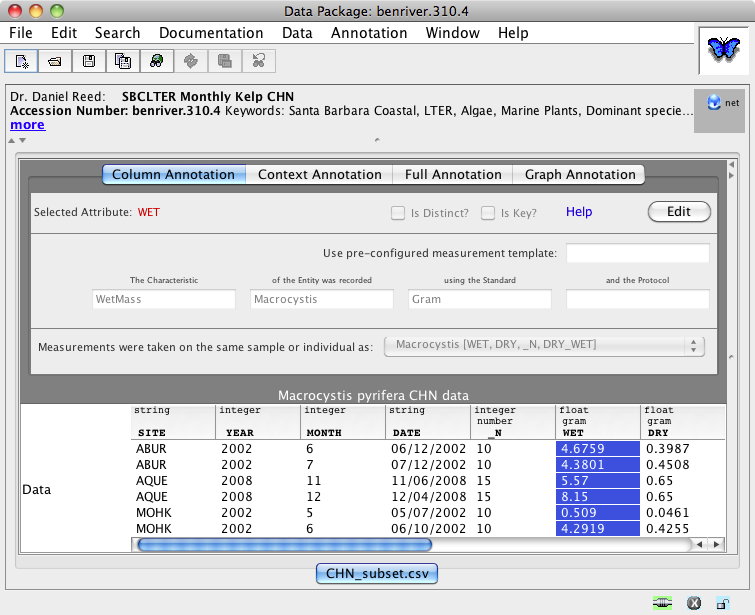
\includegraphics[width=0.5\textwidth]{images/morpho-annotation.png}
\caption{Morpho metadata editor with Semantic plugin. Fill-in-the-blank style editing interface to encourage natural language descriptions. A searchable hierarchical browser is used to select concepts from an ontology.}
\label{fig:morpho-annotation}
\end{figure}

\subsection{Metacat query extensions}
The semantic plugin for Metacat augements existing metadata storage and search by allowing Annotations to be saved and queried alongside the metadata and data that they annotate. In addition to traditional keyword and spatial search criteria, the Metacat plugin allows semantic criteria to be included where they may either increase query recall using term-expansion (i.e. traversing the class subsumption hierarchy) or refine the resultset by limiting matches to datasets that contain the specified observational model (e.g. combinations of OBOE-compatible Entity, Characteristic, or Protocol concepts). The observational model can be leveraged further by materializing the Annotation and data artifact (via the Data Manager Library) into a full OBOE model and inspecting the observational values themselves. 

%%% Local Variables: 
%%% mode: latex
%%% TeX-master: "main"
%%% End: 
